\documentclass[12pt,a4paper]{article}
% 如果需要中文支持，推荐使用xeCJK + 字体设置
% \usepackage{xeCJK}
% \setCJKmainfont{SimSun}  % 示例：宋体，可根据系统字体情况更换
\usepackage{ctex}
\setlength{\parindent}{2em}
\setlength{\parskip}{0pt} % 确保段落之间没有额外的空行间距


\usepackage{amsmath}      % 数学公式（如有需要）
\usepackage{graphicx}     % 插图
\usepackage{geometry}     % 调整页边距
\usepackage{fancyhdr}     % 自定义页眉页脚
\usepackage{indentfirst}  % 中文首行缩进
\usepackage{calc}         % 允许做长度运算(测量文字宽度等)
\usepackage{titlesec}
\usepackage{booktabs} % 解决 \midrule 和 \bottomrule 报错
\usepackage{enumitem} % 支持自定义列表格式
\usepackage{float}    % 支持强制浮动位置
\usepackage{siunitx}
\usepackage{wrapfig}

% 设置 \section 级标题为：加粗、大字号（如 \Large）
\titleformat{\section}
	{\bfseries\large}    % 标题自身的格式
	{\thesection}        % 标题编号的显示方式
	{1em}                % 编号与标题文字之间的间距
	{}                   % 在标题文字前后可插入额外代码，此处为空
	
% 设置 \subsection 级标题为：加粗、中等字号（如 \normalsize）
\titleformat{\subsection}
	{\bfseries\normalsize}
	{\thesubsection}
	{1em}
{}

% 页面设置（可根据需要微调）
\geometry{
	left=2cm,
	right=2cm,
	top=1cm,
	bottom=1.5cm
}

% 不需要过大的行距，使用较接近单倍行距的设置
\renewcommand{\baselinestretch}{1.2}

% 仅在页脚居中显示页码，页眉保持为空
\pagestyle{fancy}
\fancyhf{}  % 清空默认的页眉页脚
\fancyfoot[C]{\thepage}
\renewcommand{\headrulewidth}{0pt}
\renewcommand{\footrulewidth}{0pt}

% 首行缩进2字符(中文习惯)
% \setlength{\parindent}{0pt}
\setlength{\leftskip}{2em}
\setlength{\parindent}{2em}

\begin{document}
	%-------------------------------------------------------
	% 1 并排两个minipage：左标题、右校徽
	%   - 0.65\textwidth + 0.35\textwidth = \textwidth
	%   - 如果校徽过大或过小，可改宽度，如 0.25\textwidth、0.3\textwidth 等
	%   - 如果想让标题更大，可将 \Huge 改成 \huge 或 \LARGE
	%-------------------------------------------------------
	\noindent
	\hspace{-2em}
	\begin{minipage}[c]{0.65\textwidth}
		\raggedright
		{\fontsize{35pt}{55pt}\selectfont 物理实验报告}
	\end{minipage}
	\begin{minipage}[c]{0.35\textwidth}
		\raggedleft
		% 强制把校徽拉大到 0.35\textwidth 宽度 (高度自动匹配)
		% 若想指定高度,可用 "height=3cm" 等. 二选一即可.
		
\includegraphics[width=\linewidth, trim={20cm 20cm 20cm 20cm}, clip]{university_logo.png}
	\end{minipage}

	\vspace{-1em}
	

	%下方画两条分割线，并在两线之间写学号、姓名、日期、时间
	
	\hrule
	\vspace{0.6em}
	\noindent
	\begin{tabular}{l l l l}
    学号：12411434 & 姓名：{郑宇轩} &
    日期：2025.10.24 & 时间：周五下午
	\end{tabular}
	\vspace{0.4em}
	\par
	\hrule

	
	\section*{\textbf{一. 实验名称：空气比热容比的测定}}
	
	\section*{\textbf{二. 实验目的}}
	\begin{enumerate}
		\item 用绝热膨胀法测定空气的比热容比。
		\item 观测热力学过程中状态变化及基本物理规律。
	\end{enumerate}

	\section*{\textbf{{三. 实验原理}}}

	
	理想气体的压强$P$、体积$V$和温度$T$在准静态绝热过程中，遵守绝热过程方程：$PV^\gamma = C$，其中 $C$ 为常数，$\gamma$是气体的定压比热容$C_P$和定容比热容$C_V$之比。也称$\gamma=\dfrac{C_P}{C_V}$为该气体的比热容比（亦称绝热指数）。理想状态下双原子分子气体的绝热指数 $\gamma = 1.4$。如图1所示，我们以贮气瓶内空气（近似为理想气体）作为研究的热学系统，进行如下实验过程：

	\begin{figure}[H]
		\centering
		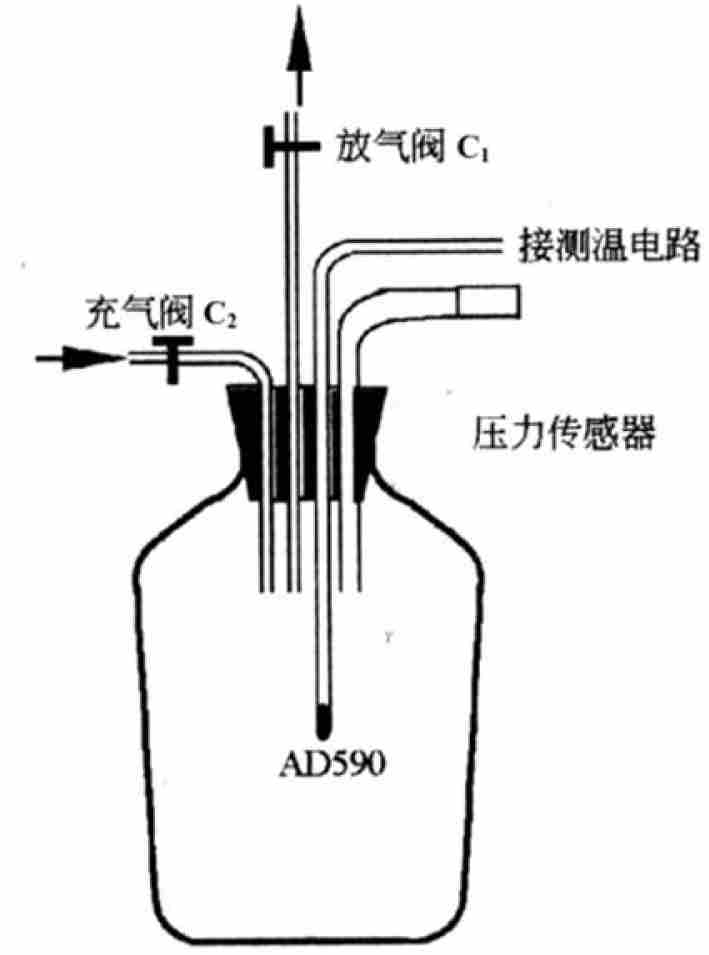
\includegraphics[width=5cm]{1.jpg}
		\caption{实验装置图}
	\end{figure}

	\begin{enumerate}
		\item 首先打开放气阀$C_1$，贮气瓶与大气相通，再关闭$C_1$，瓶内充满与周围空气同温（设为$T_0$）同压（设为$P_0$）的气体；
		\item 打开充气阀$C_2$用充气球向瓶内打气，充入一定量的气体，然后关闭充气阀$C_2$。此时瓶内空气被压缩，压强增大，温度升高。等待内部气体温度稳定，即达到与周围温度平衡，此时的研究的气体处于状态\uppercase\expandafter{\romannumeral1}$(P_1,V_1,T_0)$。虽然瓶内气体的体积为贮气瓶容积$V_0$，而仅有$V_1$部分（$V_1<V_0$）是实验研究的对象，如图2；
		\item 迅速打开放气阀$C_1$，使瓶内气体与大气相通，当瓶内压强降至$P_0$时，立刻关闭放气阀$C_1$将有体积为$\Delta V$的气体喷泻出贮气瓶。由于放气过程较快，瓶内保留的气体来不及与外界进行热交换，可以认为是一个绝热膨胀的过程。在此过程后瓶中的气体由状态\uppercase\expandafter{\romannumeral1}$(P_1,V_1,T_0)$转变为状态\uppercase\expandafter{\romannumeral2}$(P_0,V_0,T_1)$。$V_0$为贮气瓶容积，$V_1$为保留在瓶中这部分气体在状态\uppercase\expandafter{\romannumeral1}$(P_1,T_0)$时的体积；
		\item 由于瓶内气体温度$T_1$低于室温$T_0$，所以瓶内气体慢慢从外界吸热，直至 达到室温$T_0$为止，此时瓶内气体压强也随之增大为$P_2$。则稳定后的气体状态为\uppercase\expandafter{\romannumeral3}$(P_2,V_0,T_0)$；从状态\uppercase\expandafter{\romannumeral2}到状态\uppercase\expandafter{\romannumeral3}的过程可以看作是一个等容吸热的过程。
	\end{enumerate}
	
	\begin{figure}[H]
		\centering
		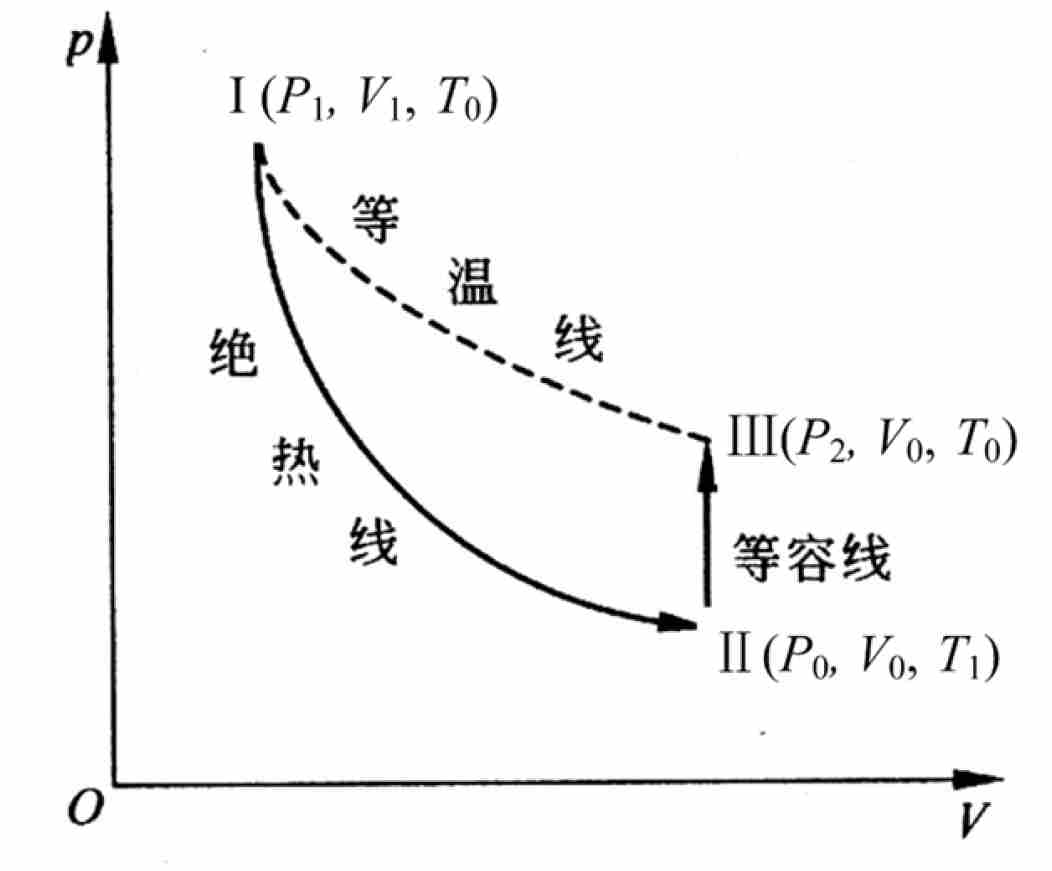
\includegraphics[scale=0.5]{2.jpg}
		\caption{气体状态变化及$P-V$图}
	\end{figure}

	由状态\uppercase\expandafter{\romannumeral1}$\rightarrow $\uppercase\expandafter{\romannumeral2}$\rightarrow $\uppercase\expandafter{\romannumeral3}的过程如图2所示。\uppercase\expandafter{\romannumeral1}$\rightarrow $\uppercase\expandafter{\romannumeral2}是绝热过程，由绝热过程方程
	得：
	\begin{align}
		P_1V_1^\gamma=P_0V_0^\gamma
	\end{align}
	状态\uppercase\expandafter{\romannumeral1}和状态\uppercase\expandafter{\romannumeral3}的温度均为$T_0$，由气体状态方程得：
	\begin{align}
		P_1V_1=P_2V_0
	\end{align}
	合并式$(1)(2)$，消去$V_0,V_1$，得：
	\begin{align}
		\gamma=\dfrac{\ln{P_1}-\ln{P_0}}{\ln{P_1}-\ln{P_2}}=\dfrac{\ln{(P_1/P_0)}}{\ln{(P_1/P_2)}}
	\end{align}
	由式$(3)$可以看出，只要测得$P_0,P_1,P_2$就可求得空气的绝热指数$\gamma$。本实验气瓶内的气压通过扩散硅传感器来测量，压强值通过电压值来显示，其灵敏度为$20\,\mathrm{mV/kPa}$。当待测压强为大气压$P_0$时将电压示数调零，当压强显示读数为$P/\mathrm{mV}$时，实际压强为：
	\begin{align}
		P(\mathrm{Pa})=P_0+50\times P(\mathrm{mV})
	\end{align}
	气瓶内温度通过AD590温度传感器测量，也是以电压值来显示，其灵敏度为$5\mathrm{mV}/^{\circ}\mathrm{C}$，最小可检测$0.02^{\circ}\mathrm{C}$的温度变化。
	
	\section*{\textbf{{四. 实验仪器}}}
	空气比热容测定仪(含 AD590 温度传感器和扩散硅压力传感器)，温度计，气压计

	\section*{\textbf{{五. 实验内容}}}

	\begin{enumerate}
    \item 用气压计测定大气压强$P_0(\text{Pa})$，用温度计测环境室温$T_0(^{\circ}\mathrm{C})$。打开放气阀$C_1$，开启电源，让电子仪器部件预热一段时间，然后将压强指示值调到“$0$”，并记录此时温度指示值$T_0$(以$\mathrm{mV}$为单位)。
    \item 关闭放气阀$C_1$，打开充气阀$C_2$，用充气球向瓶内打气，使压强升高到$100\,\mathrm{mV}-120\,\mathrm{mV}$。然后关闭充气阀$C_2$，当瓶内气体压强和温度的指示值不变时，气体处于状态\uppercase\expandafter{\romannumeral1}，记下压强$P_1$和温度$T_1$（以$\mathrm{mV}$为单位）。
    \item 迅速打开放气阀$C_1$，当放气声消失时立刻关闭放气阀$C_1$，此时瓶内空气压强降至大气压强$P_0$，气体温度降低，气体处于状态\uppercase\expandafter{\romannumeral2}。
    \item 待瓶内气体的温度上升稳定，且压强也稳定后，此时瓶内气体近处于状态\uppercase\expandafter{\romannumeral3}，记录压强$P_2$和温度$T_2$。
    \item 打开放气阀$C_1$使贮气瓶与大气相通，以便于下一次测量。
    \item 重复步骤$2-4$，重复$10$次测量，比较多次测量中气体的状态变化有何异同，并计算$\overline{\gamma}$，分析误差，利用统计规律公式$\sqrt{\dfrac{\sum_{i=1}^{n}(x_i-\overline{x})^2}{n-1}}$，计算实验结果的随机涨落偏差。
    \item 放气时间过长，重复步骤$2-4$，重复$5$次测量，计算$\overline{\gamma_1}$。
    \item 放气时间不充分，重复步骤$2-4$，重复$5$次测量，计算$\overline{\gamma_2}$。
    \item 比较三种情况的测量平均值，与理论值$1.40$比较，计算与理论值对比的相对误差$E_r=\dfrac{\overline{\gamma_i}-1.40}{1.40}\times100\%$，并分析偏离原因。
\end{enumerate}
	
	\section*{\textbf{{六. 数据记录}}}
	
	原始测量数据见附表 1。

	\section*{\textbf{{七. 数据处理}}}

	\begin{enumerate}
		\item \textbf{计算各组实验绝热指数}
		
		实验开始时大气压 $P_1 = 100780\mathrm{Pa}$，结束时 $P_2 = 100720\mathrm{Pa}$，取平均值得到 $P_0 = 100750\mathrm{Pa}$。

		实验开始时环境温度 $T_1 = 25.5^{\circ}\mathrm{C}$，结束时 $T_2 = 25.9^{\circ}\mathrm{C}$。

		双原子分子绝热指数参考值 $\gamma_0 = 1.40$

		计算每次实验测得的绝热指数 $\gamma$，结果如下图：

		\begin{figure}[H]
			\centering
			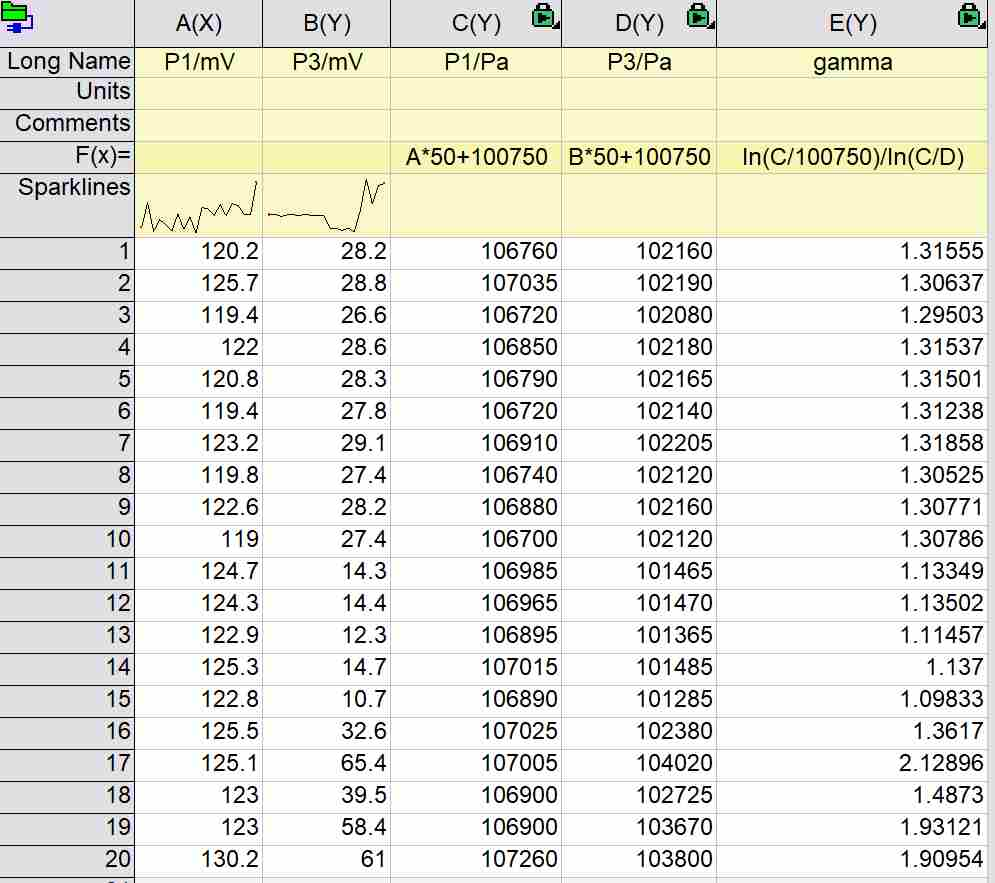
\includegraphics{3.jpg}
			\caption{各组实验绝热指数}
		\end{figure}

		\item \textbf{计算平均值与误差}
		
		\textbf{正常放气时间}
		
		绝热指数平均值

		$$\bar{\gamma} = \dfrac{1}{10}\sum_{i=1}^{10}\gamma_i = \dfrac{1.316+1.306+\cdots + 1.308}{10} = 1.310$$

		相对误差

		$$\epsilon = \dfrac{|\bar{\gamma} - \gamma_0|}{\gamma_0} \times 100\% = \dfrac{1.310 - 1.40}{1.40} \times 100\% = 6.43\%$$

		随机涨落偏差

		$$S_{\bar{\gamma}} = \sqrt{\dfrac{\sum_{i=1}^{n}(\gamma_i-\bar{\gamma})^2}{n-1}} = \sqrt{\dfrac{(1.316-1.310)^2+(1.306-1.310)^2+\cdots +(1.308-1.310)^2}{10-1}} = 0.007$$
		
		\textbf{放气时间过短}

		绝热指数平均值

		$$\bar{\gamma_1} = \dfrac{1}{5}\sum_{i=11}^{15}\gamma_i = \dfrac{1.133+1.135+\cdots + 1.110}{5} = 1.124$$

		远小于理论值 $\gamma_0 = 1.40$，此时相对误差

		$$\epsilon_1 = \dfrac{|\bar{\gamma_1} - \gamma_0|}{\gamma_0} \times 100\% = \dfrac{1.124 - 1.40}{1.40} \times 100\% = 19.71\%$$

		\textbf{放气时间过长}
		
		绝热指数平均值

		$$\bar{\gamma_2} = \dfrac{1}{5}\sum_{i=16}^{20}\gamma_i = \dfrac{1.362+2.129+\cdots + 1.910}{5} = 1.764$$

		远大于理论值 $\gamma_0 = 1.40$，此时相对误差

		$$\epsilon_2 = \dfrac{|\bar{\gamma_2} - \gamma_0|}{\gamma_0} \times 100\% = \dfrac{1.764 - 1.40}{1.40} \times 100\% = 26.00\%$$

	\end{enumerate}

	
	\section*{\textbf{八. 误差分析}}

	\begin{enumerate}
		\item 实验过程中因装置漏气更换实验装置，可能导致实验结果不一致；
		\item 温度传感器和压力传感器的灵敏度有限，可能导致测量误差；
		\item 无法精准控制放气时间，放气时间过长或过短都会影响实验结果；
		\item 装置无法完全绝热，气体在放气以及等待平衡过程中与外界有热交换，影响了实验结果；
		\item 实验前后的气压与温度有变化，可能导致实验结果不准确；
		\item 平衡过程时间较长，可能提前读取结果导致结果不准确；
		\item 气体不是理想气体，实际气体的行为与理想气体有所不同，可能导致实验结果偏差。
	\end{enumerate}

	\section*{\textbf{{九. 问题思考}}}

	\begin{enumerate}
		\item \textbf{写出等精度测量实验的定义。这个实验是等精度测量吗？请简述理由。}

		等精度测量是指在测量条件保持不变的情况下，对同一被测量进行多次重复测量的过程，其中实验对象、测量方法、测量设备、实验环境、实验人员等条件在理想状态下均不发生改变。
		
		该实验不是等精度实验。因为在每次重复实验中，环境温度都会发生变化，无法保证实验环境不发生改变。
		
		\item \textbf{为什么在实验中不需要测量状态 II 的压强和温度值？请简述理由。}
		
		状态\uppercase\expandafter{\romannumeral2}不是稳态，无法精准测量；并且由公式$(3)$，计算$\gamma$时不需要状态\uppercase\expandafter{\romannumeral2}的压强和温度，故无需测量。
		
	\end{enumerate}

	
	\section*{\textbf{{十. 实验结论}}}

	本实验使用绝热膨胀法，测定空气的比热容比。
	
	在放气时间正常、放气时间过长、放气时间过短三种情况下，分别测得放气时间正常时的比热容比为$\overline{\gamma}=1.310$，相对误差为 $6.43 \%$，此时随机涨落偏差为 $0.007$，处于合理范围；放气时间过长时的比热容比为$\overline{\gamma_1}=1.124$，相对误差为 $19.71 \%$；放气时间不充分时的比热容比为$\overline{\gamma_2}=1.764$，相对误差为 $26.00 \%$。本实验发现放气时间过长或过短均会误差较大，而正常放气时误差较小。

\end{document}